\chapter{Risultati}
\vspace{4cm}

Riportiamo ora i tempi medi di runtime ottenuti eseguendo dei test con la
versione Rectangular su un dataset di 4096 elementi eseguito per 15 volte su
ognuno dei seguenti dispositivi:

Si riportano di seguito i tempi di runtime ottenuti eseguendo dei test su dataset di diverse dimensioni e caratteristiche generati attraverso il generatore descritto al capitolo 4.

Si sono effettuate 20 esecuzioni dell'algoritmo per ogni dataset, sia su GPU NVIDIA GeForce GTX 1650 che su CPU Intel(R) Core(TM) i7-10710U CPU @ 1.10GHz.



\subsection{Confronto tra prestazioni attese e prestazioni effettive}
Tenendo conto dei dati teorici riguardanti la memory bandwidth delle varie piattaforme possiamo provare a determinare se questo algoritmo riesce effettivamente a sfruttare tutti i device allo stesso modo oppure se qualcuno di questi performa meno di quanto dovrebbe.

In particolare le memorie dei Device su cui sono stati eseguiti i test hanno banda passante teorica pari a:
\begin{enumerate}
	\item Dedicata: $\SI{121.1}{\giga\byte/\second}$
	\item CPU: $\SI{15.0}{\giga\byte/\second}$ (Dovuta al bus PCIe 3.0)
\end{enumerate}
da cui ne deriva una ratio pari a circa $16/3$ tra Dedicata e CPU.

I valori del test ottenuti con la versione \textit{Rectangular} vettorizzata mostrano invece una ratio di circa $20/9$ calcolata facendo una stima dei byte letti e scritti in media dai kernel e dividendo questa cifra per il tempo di runtime.

Ne deduciamo che la GPU non è effettivamente sfruttata a pieno e che probabilmente le cause di questa mancanza sono da ricercare nella frammentazione della coda dei task da analizzare e nei trasferimenti di memoria con l'host necessari a terminare l'iterazione del kernel.

Il primo di questi problemi è dovuto al fatto che la coda, nella sua implementazione attuale, contiene un valore non nullo nelle posizioni dell'array che corrispondono ai nodi da analizzare. Per ovviare a questo problema si potrebbe pensare di usare una coda effettiva invece di un array, tuttavia questo non è possibile perché i workitem dovrebbero sincronizzarsi per decidere a quale indirizzo poter inserire il nuovo nodo da aggiungere alla coda.

Anche il secondo problema come discusso in precedenza non è risolvibile a causa dell'impossibilità di sincronizzare workitem di workgroup diversi.



\subsection{Andamento delle prestazioni}
Si riportano i risultati dei test eseguiti su una GPU NVIDIA GTX 1650 con dataset di varia grandezza. Per ogni dataset sono state eseguite 15 iterazioni con la versione \textit{Rectangular} vettorizzata dei kernel e successivamente sono stati calcolati i tempi medi di runtime:


\begin{figure}[H]
	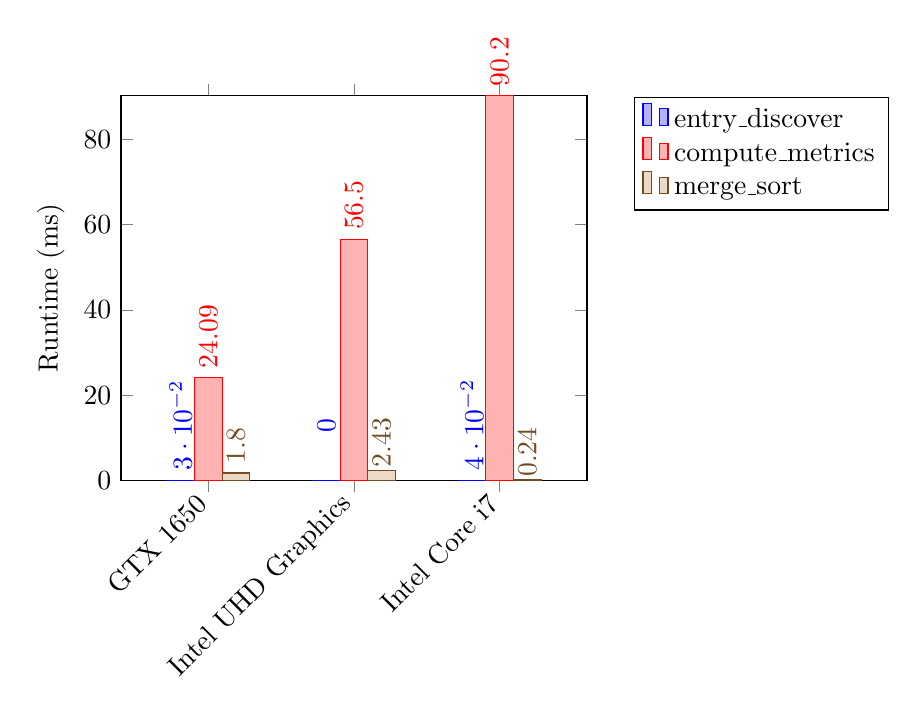
\begin{tikzpicture}
		\begin{axis}[
			symbolic x coords={
				GTX 1650,
				Intel UHD Graphics,
				Intel Core i7
			},
			xtick=data,
			x tick label style={rotate=45,anchor=east},
			nodes near coords,
			every node near coord/.append style={rotate=90, anchor=center},
			ylabel=Runtime (ms),
			legend style={at={(1.1, 0.85)}, anchor=west},
			ybar=0pt,
			legend cell align={left},
			enlarge x limits=0.3,
			enlarge y limits=0,
			width=7.5cm,
			]
			\addplot+[every node near coord/.append style={yshift=10pt, xshift=30pt}] coordinates { %entries discover
				(GTX 1650, 0.03)
				(Intel UHD Graphics, 0.00)
				(Intel Core i7, 0.04)
			};
			\addplot+[every node near coord/.append style={xshift=0pt, anchor=west}] coordinates { %compute metrics
				(GTX 1650, 24.09)
				(Intel UHD Graphics, 56.50)
				(Intel Core i7, 90.20)
			};
			\addplot+[every node near coord/.append style={yshift=-10pt, xshift=0pt}] coordinates { %mergesort
				(GTX 1650, 1.80)
				(Intel UHD Graphics, 2.43)
				(Intel Core i7, 0.24)
			};
			\legend{entry\_discover, compute\_metrics, merge\_sort}
		\end{axis}
	\end{tikzpicture}
	\caption{Tempi di runtime della versione \textit{Rectangular} vettorizzata}
\end{figure}